\documentclass[9pt]{exam}
\usepackage[utf8]{inputenc}
\usepackage{amsmath,amsthm,amsfonts,amssymb,amscd}
\usepackage{multirow,booktabs}
\usepackage{enumitem}
\usepackage{fancyhdr}
\usepackage{mathrsfs}
\usepackage{wrapfig}
\usepackage{setspace}
\usepackage{calc}
\usepackage{multicol}
\usepackage{cancel}
\usepackage[retainorgcmds]{IEEEtrantools}
\usepackage{framed}
\usepackage[most]{tcolorbox}
\usepackage{tikz}
\usepackage{geometry}
\geometry{
	a4paper,
	total={170mm,257mm},
	left=20mm,
	top=20mm,
}
\title{Electromagnetism}
\author{Aaron G.K.}
\begin{document}
	\maketitle
	\section*{Magnetism}
	Magnetism is an important phenomenon that we experience almost everyday. It is also one of the most ancient historical perceptions in physics and was discovered early on in history. As you have probably studied in earlier grades, the idea of magnetism goes a long way - and perhaps it is one of the oldest physical phenomena discovered. The phenomenon first being recorded dates back before the birth of Christ, particularly in a region of Asia Minor called Magnesia (the name of this region is the source of words like \textit{\textbf{magnetic}}). Magnetic rocks found in Magnesia, which is now part of western Turkey, stimulated interest during ancient times. The use of magnets in compasses - their earliest application - resulted not just in improved expeditions, but also in the names of “north” and “south” being given to the two types of magnetic poles. \\ \\
	\begin{center}
		\includegraphics*[scale=0.5]{aurora_borealis}
	\end{center}
	\textit{The magnificent spectacle of the Aurora Borealis, or northern lights, glows in the northern sky above Bear Lake near Eielson Air Force Base, Alaska. Shaped by the Earth’s magnetic field, this light is produced by radiation spewed from solar storms.} \\ \\
	Magnetism plays a great role in the human civilization - it would not be an overstatement to say civilization would not exist if not for a great role played by magnetism. For instance, electric motors, with uses as diverse as powering refrigerators, starting cars, and moving elevators, contain magnets. Generators, whether producing hydroelectric power or running bicycle lights, use magnetic fields. In addition, magnetism play a great role in different fields such as the medical field in Magnetic resonance imaging (MRI) - which has become an important diagnostic tool in the medical field.
	\section*{Magnets}
	So, we now understand that magnets are very useful and also cause a lot of beautiful phenomenon on the sky! But, let's take a look at the common magnets we have around us. You probably have seen many types of magnets in your earlier grades, mainly categorized based on shape.
	\begin{center}
		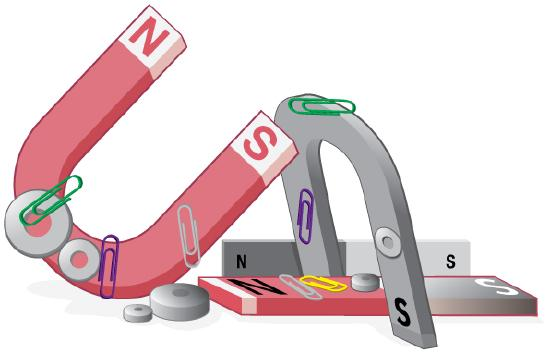
\includegraphics[scale=0.5]{magnets}
	\end{center}
	We can see in the figure above, that the magnets attract other metals such as paperclips around them, and also another important fact - no matter the shape or size of the magnets, they always have two poles - the North \& South poles. So, magnets can come in different sizes or shapes, but they always have two poles. Recall the similarity this has with charges having dual polarities(negative \& positive). However, we can never have a magnetic monopole - a North or South pole alone. Another that magnets have with charges is that like poles repel while unlike poles attract. \\ \\ To summarize:
	\begin{itemize}
		\item Similar to charges, magnets have dual poles - North \& South
		\item Similar to charges, the like poles repel while the unlike poles attract
	\end{itemize}
	\section*{Earth's Magnetic Field}
	Although the origin of Earth's magnetic field remains fairly a mystery, we can logically hypothesize and explain the phenomenon within scientific reason. One major hypothesis is that the Earth's magnetic field is mostly caused by electric currents in the liquid outer core. 
	\begin{center}
		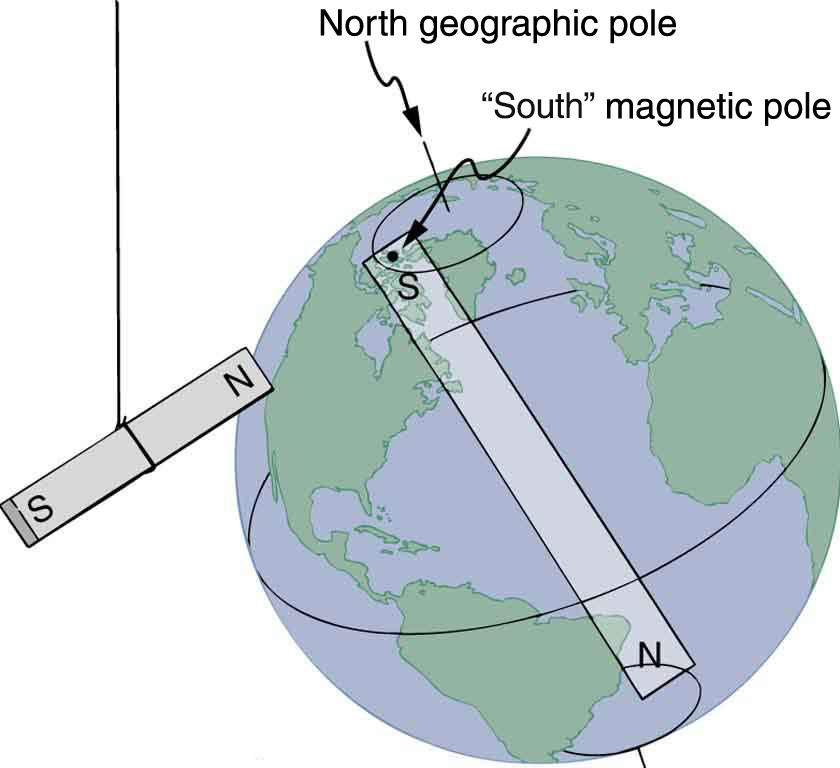
\includegraphics[scale=0.2]{earth_magnetic_field}
	\end{center}
	We can effectively think of the magnetic field of the Earth as being caused by a large bar magnet inside the Earth. That way, we can just assume the globe of the Earth with a bar magnet inside it. The south pole of the bar magnet inside the globe is is near, but not exactly on, the north geographic pole. The north pole of the bar magnet inside the globe is near the south geographic pole. \\ \\
	\subsection*{A Compass}
	\begin{center}
		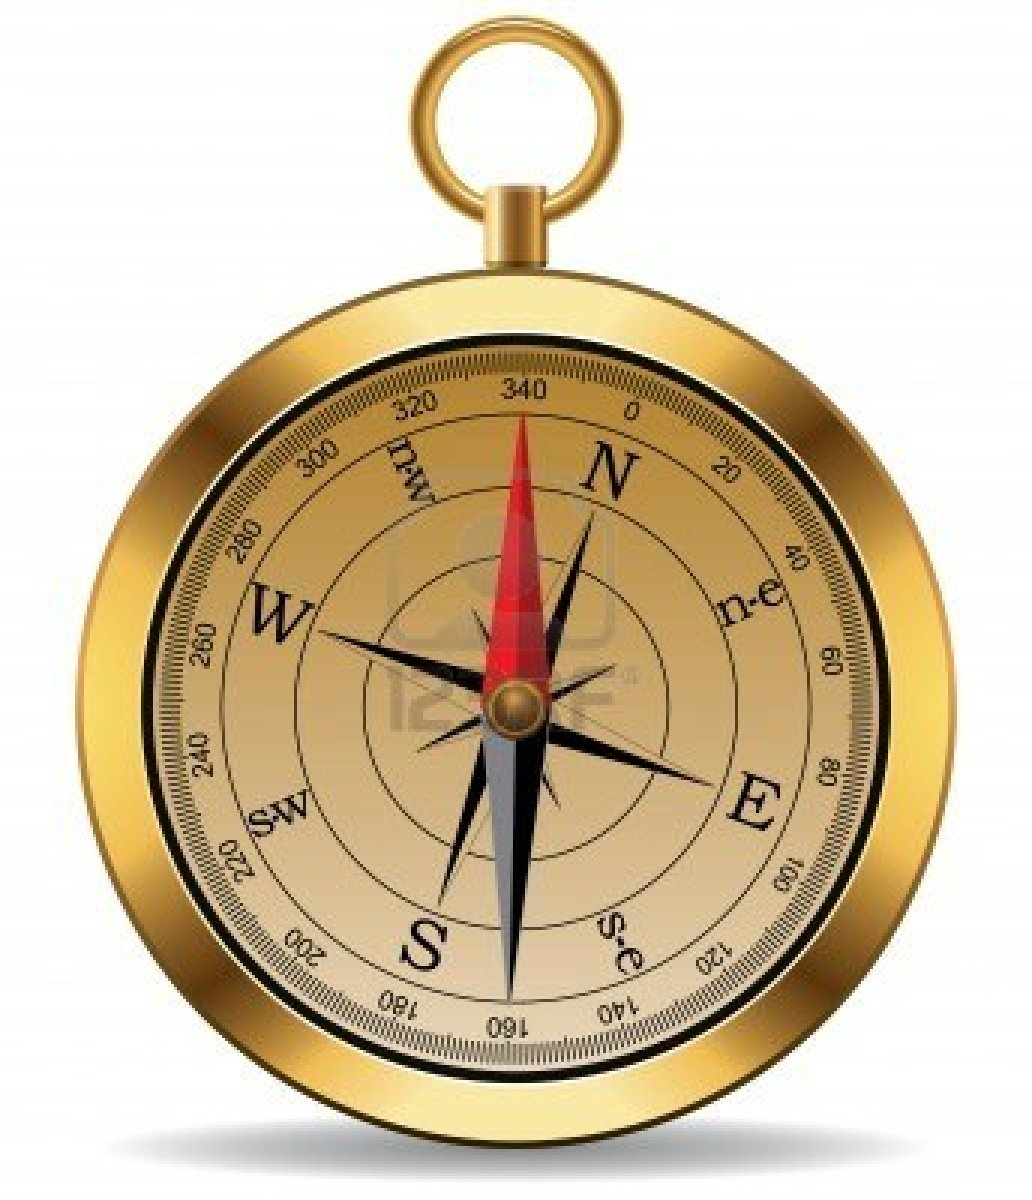
\includegraphics[scale=0.1]{compass}
	\end{center}
	A compass is an instrument which is used to find the direction of a magnetic field. It can do this because a compass consists of a small metal needle which is magnetized itself and which is free to turn in any direction. Therefore, in the presence of a magnetic field, the needle is able to line up in the same direction as the field. Compasses are mainly used in navigation to find direction on the earth. This works because the earth itself has a magnetic field which is similar to that of a bar magnet shown above. The compass needle aligns with the magnetic field direction and points north (or south). Once you know where north is, you can figure out any other direction. \\ \\
	If we have a compass, such as on the figure above; the north pole of this magnet is pointing toward the north pole of the globe (or the south pole of the magnet inside the globe). The Earth acts like a very large bar magnet with its south-seeking pole near the geographic North Pole. That is why the north pole of a compass is attracted toward the geographic north pole of the Earth — because the magnetic pole that is near the geographic North Pole is actually a south magnetic pole. \\ \\ \textbf{\textit{Confusion arises because the geographic term “North Pole” has come to be used (incorrectly) for the magnetic pole that is near the North Pole. Thus, “North magnetic pole” is actually a misnomer—it should be called the South magnetic pole.}}
	\section*{Types of Magnets}
	We can categorize magnets in various ways. We can categorize them based on shape, for example. We have many different shapes of magnets: ring, bar, cylindrical, arc, etc. However, we can categorize magnets based on longevity as well:
	\begin{itemize}
		\item \textbf{Permanent Magnets}: are made up of ferromagnetic materials that are magnetized and have their own magnetic fields.	They are known as permanent magnets because they do not lose their magnetic property once they are magnetized. However, the strength depends upon the nature of the material used in its creation.
		\item \textbf{Temporary Magnets}: can be magnetized in the presence of a magnetic field. When the magnetic field is removed, these materials lose their magnetic property. Iron nails and paper-clips are examples of the temporary magnet.
		\item \textbf{Electromagnets}: consist of a coil of wire wrapped around the metal core made from iron. When the coil of wire conducts a current, a magnetic field is generated making the material behave like a magnet. The strength of the magnetic field can be controlled by controlling the electric current. Electromagnets are used in the generators, motors, transformers, loudspeakers, MRI machines, magnetic locks etc.
	\end{itemize}
	\section*{More on Ferromagnetic Substances and Electromagnets}
	The fact that magnetic poles always occur in pairs of north and south is true from the very large scale—for example, sunspots always occur in pairs that are north and south magnetic poles—all the way down to the very small scale. Magnetic atoms have both a north pole and a south pole, as do many types of subatomic particles, such as electrons, protons, and neutrons. Recall earlier that we have seen we can never have a magnetic monopole.
	\begin{center}
		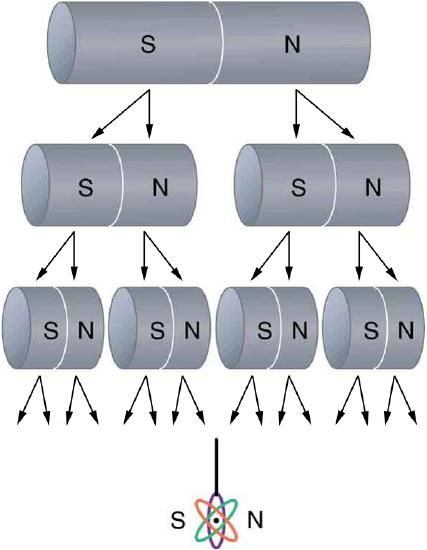
\includegraphics[scale=0.3]{magnets_divided}
	\end{center}
	From the above concept, we can deduce all magnets are made up of smaller magnets. These smaller magnets are called magnetic domains. We know that magnets can only be made of certain materials - these materials are called  ferromagnetic. Ferromagnetic materials are materials that are able to be magnetized. Common examples of elements that are ferromagnetic include iron, nickel, cobalt, and gadolinium. The difference between the magnets and the ferromagnetic materials that aren't magnets yet is the arrangement of the magnetic domains.
	\begin{center}
		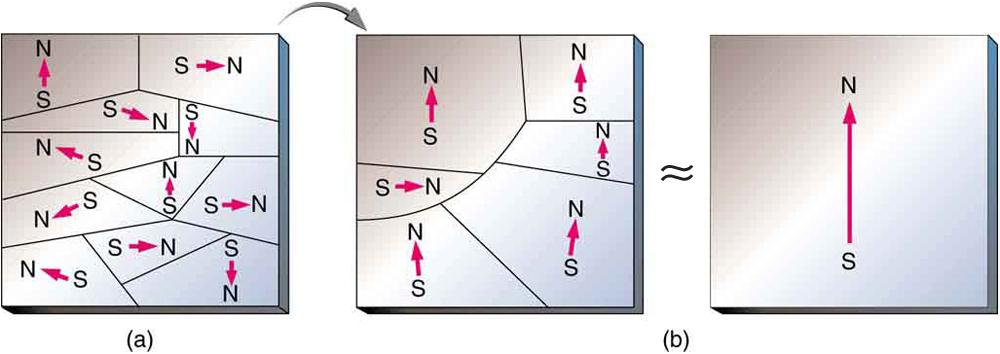
\includegraphics[scale=0.2]{magnetic_domains}
	\end{center}
	In Figure \textbf{a}, there are many domains but each domain has a slightly different orientation. In Figure \textbf{b}, the domains are larger. Most of the domains are oriented in roughly the same direction. In Figure \textbf{c} - which is broadly the overall effect of the figure in \textbf{b}, there is a single domain for the entire piece of iron. There is a north pole and a south pole.
	\section*{Magnetization \& Demagnetization}
	\begin{center}
		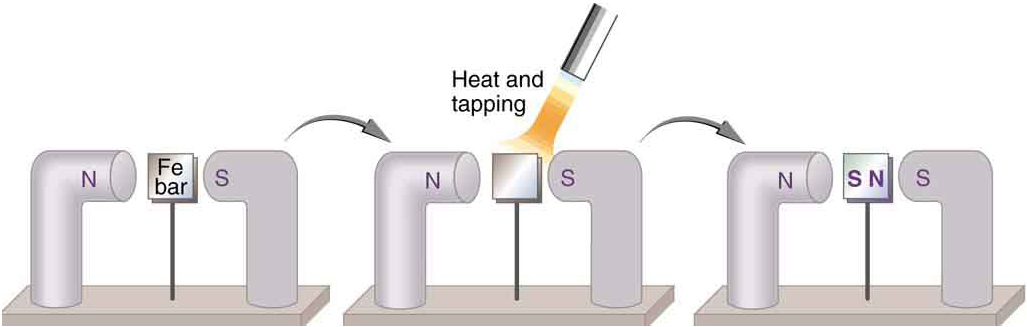
\includegraphics[scale=0.3]{magnetization}
	\end{center}
	When a magnet is brought near a previously unmagnetized ferromagnetic material, it causes a local magnetization of the material with opposite poles closest. This is due to the rearrangement of the magnetic domains. Within domains, the poles of individual atoms are aligned. Each atom acts like a tiny bar magnet. Domains are small and randomly oriented in an unmagnetized ferromagnetic object. In response to an external magnetic field, the domains may grow to millimeter size, aligning themselves in an ordered manner. This \textit{\textbf{induced magnetization can be made permanent}} if the material is heated and then cooled, or simply tapped in the presence of other magnets. Sometimes, however, magnetic effects of objects are not desired, thus we remove the magnetic effects(demagnetize) the objects. The following are the ways to demagnetize the permanent magnets:
	\begin{itemize}
		\item Exposing magnets to extreme temperatures: the temperature beyond which a ferromagnetic material loses its magnetic property is called the Curie Temperature. It is unique for each element.
		\item The magnetic attraction between the magnet’s atoms gets loosen when they are hammered.
		\item Stroking one magnet with the other in an inappropriate manner will reduce the magnetic strength.
	\end{itemize} 
	\section*{Summary}
	\begin{itemize}
		\item When a magnet is dipped in iron filings, you can observe that the iron filings cling to the end of the magnet as the attraction is maximum at the ends of the magnet. These ends are known as poles of the magnets.
		\item Magnetic poles always exist in pairs. Thus, when a magnet is cut into two pieces, both the pieces will have the North Pole and the South Pole.
		\item Whenever a magnet is suspended freely in mid-air, it always points towards north-south direction. Pole pointing towards geographic north is known as the North Pole and the pole pointing towards geographic south is known as the South Pole.
		\item Like poles repel while unlike poles attract.
		\item The magnetic force between two magnets is greater when the distance between these magnets is lesser.
	\end{itemize}
	\subsection*{Questions}
	\begin{enumerate}
		\item What is a magnet? List its properties.
		\item Does the earth have a magnet? What do you think?
		\item What is the purpose of a compass? Why does it always point to the Geographic North?
		\item What are magnetic poles? Does magnetic monopole exist? If you broke a magnet into two, would you have isolated north
		and south poles? Explain.
		\item Explain the significance of the Curie temperature.
		\item Describe the source of Earth's magnetic field.
	\end{enumerate}

\section*{Vectors}
Vectors are Euclidean quantities that have geometric representations as arrows in one dimension (in a line), in two dimensions (in a plane), or in three dimensions (in space). They can be added, subtracted, or multiplied. They are quantities that need \textit{magnitude}, \textit{direction} and a proper \textit{unit} to be adequatey expressed.
\subsection*{Representing Vectors}
Assuming a coordinate system(could be  line, plane, or even a space), we can represent vectors by writing unique directed line segments that have their initial points at the origin. They are usually described in terms of their components in a coordinate system. Even in everyday life we naturally think of the concept of perpendicular projections in a rectangular coordinate system. For example, if you ask someone for directions to a particular location, you will more likely be told to go 3km east and 4 km north than 5 km in the direction 53$^0$ north of east.\\ \\
In a an xy - coordinate system in a plane, a point in a plane is described by a pair of coordinates (x, y). In a similar fashion, a vector  $\vec{A}$ in a plane is described by a pair of its vector coordinates. The x-coordinate of vector  $\vec{A}$ is called its x-component and the y-coordinate of vector  $\vec{A}$ is called its y-component. The vector x-component is a vector denoted by  $\vec{A_x}$ while the vector y-component is a vector denoted by  $\vec{A_y}$. \\ \\
Since the x and y vector components of a vector are the perpendicular projections of the vector onto the  x and  y-axes, respectively, each vector on a Cartesian plane can be expressed as the vector sum of its vector components as follows:
$$\vec{A} = \vec{A}_{x} + \vec{A}_{y} $$
\begin{center}
	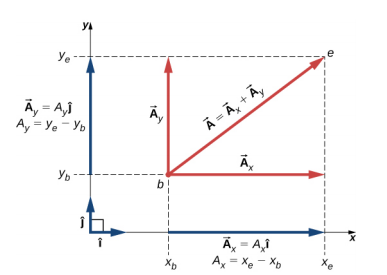
\includegraphics[scale=0.5]{cartesian_plane}
\end{center}
Since the magnitude of unit vectors is one, we usually denote the positive direction on the x-axis by the unit vector  $\hat{i}$
and the positive direction on the y-axis by the unit vector  $\hat{j}$. That means, we can describe the vectors above as follows:
$$\vec{A}_{x} = A_{x} \hat{i}$$
$$\vec{A}_{y} = A_{y} \hat{j}$$
The above implies that we can express vector $\vec{A}$ as follows:
$$\vec{A} = A_{x} \hat{i} + A_{y} \hat{j} \ldotp \label{2.12}$$
If we know the scalar components $A_x$ and $A_y$, we can find the magnitude of the vector and the direction angle that is measured (conventionally) counterclockwise from the positive x- axis. To find the magnitude, we simply use Pythagoras' theorem since $\vec{A_x}$ and $\vec{A_y}$ are orthogonal:
$$A^{2} = A_{x}^{2} + A_{y}^{2} \Leftrightarrow A = \sqrt{A_{x}^{2} + A_{y}^{2}} $$
To find the direction angle($\theta$), we can use any of the trigonometric functions, but tangent seems generally simpler. Thus,
$$\tan \theta = \frac{A_{y}}{A_{x}} \Rightarrow \theta = \tan^{-1} \left(\dfrac{A_{y}}{A_{x}}\right)$$
\subsection*{Three Dimensional Vectors}
To specify the location of a point in space, we need three coordinates (x, y, z), where coordinates x and z specify locations in a plane, and coordinate y gives a vertical positions above or below the plane. A three-dimensional space has three orthogonal directions, so instead of the two unit vectors we used earlier, we need three unit vectors to define a three-dimensional coordinate system. The third unit vector in the z direction is the $\hat{k}$ vector. The order in which the axes are labeled, which is the order in which the three unit vectors appear, is important because it defines the orientation of the coordinate system. You may see in different places the axis definitions being different. Some textbooks use the z axis as the vertical axis while others use y. It really is an arbitrary choice and it does not affect the physics.
\begin{center}
	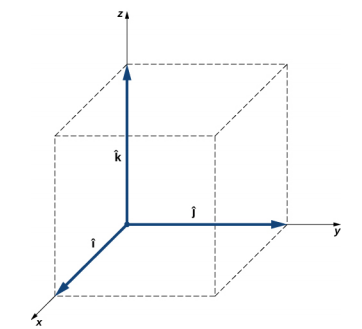
\includegraphics[scale=0.4]{cartesian_space}
\end{center}
In three-dimensional space, vector $\vec{A}$ has three vector components: the x-component $\vec{A_x}=A_x\hat{i}$, which is the part of vector $\vec{A}$ along the x-axis; the y-component $\vec{A_y}=A_y\hat{j}$, which is the part of vector $\vec{A}$ along the y-axis; the z-component $\vec{A_z}=A_z\hat{k}$, which is the part of vector $\vec{A}$ along the x-axis; A vector in three-dimensional space is the vector sum of its three vector components:
$$\vec{A} = A_{x} \hat{i} + A_{y} \hat{j} + A_{z} \hat{k}$$
To find the magnitude of our three-dimensional vector, we use the method we used above(Pythagoras' theorem) as follows. To understand, look closely at the figure below:
\begin{center}
	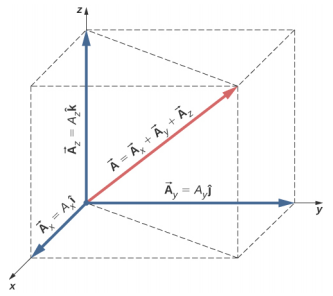
\includegraphics[scale=0.6]{resultant_3d}
\end{center}	
This makes the magnitude of $\vec{A}$ to be given as:
$$A = \sqrt{A_{x}^{2} + A_{y}^{2} + A_{z}^{2}}$$
When giving directions for three-dimensional vectors, we can't necessarily use one specific angle because there needs to be at least two angles to adequately describe the vector. The general rule of finding the unit vector  $\hat{A}$ of direction for any vector $\vec{A}$ is to divide it by its magnitude V:
$$\hat{V} = \frac{\vec{V}}{V}$$
We see from this expression that the unit vector of direction is dimensionless because the numerator and the denominator in have the same physical unit. That means, we can express the unit vector of direction in terms of unit vectors of the axes.
\section*{Vector Algebra}
\subsection*{Vector Addition}
If we express vectors in terms of the unit vectors of the coordinate axes, it simplifies a lot of things in vector algebra. Since we have the common unit vectors for all vectors we can just add the coefficients of the unit vectors to simply arrive at the result we want. While adding vectors, it is common to multiply them with scalars when doing certain calculations - \textbf{it is important to understand that multiplication of a scalar with a vector will always result in a vector that is in the same direction as the original vector}. \\ \\
For two vectors $\vec{A}$ and $\vec{B}$ such that $\vec{A}=A_{x}\; \hat{i} + A_{y}\; \hat{j} + A_{z}\; \hat{k}$ and $\vec{B}=B_{x}\; \hat{i} + B_{y}\; \hat{j} + B_{z}\; \hat{k}$, the sum of the two vectors, $\vec{R}=\vec{A}+\vec{B}$ is given by:
$$\vec{R} = \vec{A} + \vec{B} = (A_{x}\; \hat{i} + A_{y}\; \hat{j} + A_{z}\; \hat{k}) + (B_{x}\; \hat{i} + B_{y}\; \hat{j} + B_{z}\; \hat{k}) = (A_{x} + B_{x})\; \hat{i} + (A_{y} + B_{y})\; \hat{j} + (A_{z} + B_{z})\;$$
\subsection*{Product of Vectors}
A vector can be multiplied by a vector or a scalar. When a vector is multiplied by a scalar we always get a vector in the same direction as the original one. However, when a vector is multiplied by another vector, we can get a scalar, or a vector depending on the type of product we use. \\ \\
There are two kinds of products: one kind of multiplication is a type of product in which the result is a scalar - hence called the scalar(dot) product. For example, work is a scalar product of force and displacement which are both vectors. Another kind of product is one where the result is a vector - hence called a vector(cross) product. For example, in rotational motion, torque is defined as a vector product applied force and lever arm which are both vectors. 
\subsubsection*{Scalar Product}
As we have seen above, scalar product is a product of vectors whose result is scalar. The scalar product of two vectors $\vec{A}$ and $\vec{B}$ is formally defined as follows:
$$\vec{A}\; \cdot \vec{B} = AB \cos \theta\hspace{0.2in}\text{such that }\theta\text{ is the angle between the two vectors}$$
One can see that for orthogonal vectors($\theta=90^0$), the dot product of the two vectors is always 0. In the Cartesian coordinate system, scalar products of unit vectors of an axis with that of an other's is always 0 because the unit vectors of the coordinate axes are always perpendicular. That means,
$$\hat{i}\cdot\hat{j}=|\hat{i}||\hat{j}|\cos90^0=0$$
$$\hat{i}\cdot\hat{k}=|\hat{i}||\hat{k}|\cos90^0=0$$
$$\hat{j}\cdot\hat{k}=|\hat{j}||\hat{k}|\cos90^0=0$$
For the dot product of unit vectors on coordinate axes with themselves, we get the following:
$$\hat{i}\; \cdotp\; \hat{i} = i^{2} = \hat{j}\; \cdotp\; \hat{j} = j^{2} = \hat{k}\; \cdotp\; \hat{k} = 1 $$
This is always because the magnitude of the unit vectors is 1; $|\hat{i}| = |\hat{j}| = |\hat{k}|$ \\ \\
For two vectors $\vec{A}$ and $\vec{B}$ such that $\vec{A} = A_{x}\; \hat{i} + A_{y}\; \hat{j} + A_{z}\; \hat{k}\; \text{ and } \vec{B} = B_{x}\; \hat{i} + B_{y}\; \hat{j} + B_{z}\; \hat{k}$, the dot product can be given as follows:
$$\vec{A}\; \cdotp \vec{B} = (A_{x}\; \hat{i} + A_{y}\; \hat{j} + A_{z}\; \hat{k})\; \cdotp (B_{x}\; \hat{i} + B_{y}\; \hat{j} + B_{z}\; \hat{k}) \\ $$
$$= A_{x}B_{x}\; \hat{i}\; \cdotp\; \hat{i} + A_{x}B_{y}\; \hat{i}\; \cdotp\; \hat{j} + A_{x}B_{z}\; \hat{i}\; \cdotp\; \hat{k} \\ + A_{y}B_{x}\; \hat{j} \cdotp\; \hat{i} + A_{y}B_{y}\; \hat{j}\; \cdotp\; \hat{j} + A_{y}B_{z}\; \hat{j} \cdotp\; \hat{k} \\ + A_{z}B_{x}\; \hat{k}\; \cdotp\; \hat{i} + A_{z}B_{y}\; \hat{k}\; \cdotp\; \hat{j} + A_{z}B_{z}\; \hat{k}\; \cdotp\; \hat{k}$$
Since scalar products of two different unit vectors of axes give zero, and scalar products of unit vectors with themselves give one there are only three nonzero terms in this expression. It simplifies to:
$$\vec{A}\; \cdotp \vec{B} = A_{x}B_{x} + A_{y}B_{y} + A_{z}B_{z}$$
\textbf{\textit{It is extremely important to understand that $\vec{A}\; \cdotp \vec{B}$ is a scalar quantity.}} \\ \\
From our primary definition of a scalar product, we know that $\vec{A}\; \cdot \vec{B} = AB \cos \theta\hspace{0.2in}$ but we have also seen have that the scalar product can be expressed in terms of the components is $\vec{A}\; \cdotp \vec{B} = A_{x}B_{x} + A_{y}B_{y} + A_{z}B_{z}$. Thus, we have 
$$ AB \cos \theta\hspace{0.2in} = A_{x}B_{x} + A_{y}B_{y} + A_{z}B_{z}$$
This means, 
$$\cos \theta  = \dfrac{A_{x}B_{x} + A_{y}B_{y} + A_{z}B_{z}}{AB} \ldotp \label{2.34}$$
\subsubsection*{Vector Product}
Vector product is a type of product between vectors that results in a vector. The vector product of two vectors $\vec{A}$ and $\vec{B}$ is formally defined as follows:
$$|\vec{A}\; \times \vec{B}| = AB \sin \theta\hspace{0.2in}\text{such that }\theta\text{ is the angle between the two vectors}$$
It is important to know that the cross product of two vectors is a \textbf{vector} that is perpendicular to both vectors that were multiplied. That's why in the above equation, we can express the magnitude of the cross product and not the vector product itself. Had we wanted to describe the vector product, we could define a unit vector that is in the direction of the vector product and use it as follows:
$$\vec{A}\; \times \vec{B}= AB\sin\theta\hat{\textbf{n}}$$
Where $\hat{\textbf{n}}$ is a unit vector in the direction of $\vec{A}\; \times \vec{B}$ and is perpendicular to both $\vec{A}$ and $\vec{B}$. \\ \\
Unlike dot products, cross products tend to result in vectors and are a little more complex to compute. From the definition, above we can see that the vector product of a vector with itself is always 0 since the sine of 0 is 0. Let's elaborate more here:
$$\hat{i} \times \hat{i} = \hat{j} \times \hat{j} = \hat{k} \times \hat{k} = 0 $$
To simplify the work, let's introduce a simple figure to visualize how it works:
\begin{center}
	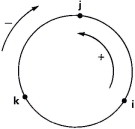
\includegraphics[scale=1.2]{cross_product_circle}
\end{center}
While we are going counterclockwise on the schematic visualizer above, we get the following
$$\begin{cases} \hat{i} \times \hat{j} = + \hat{k}, \\ \hat{j} \times \hat{k} = + \hat{i}, \\ \hat{k} \times \hat{i} = + \hat{j} \ldotp \end{cases}$$
Similarly, going clockwise, we get
$$\begin{cases} \hat{j} \times \hat{i} = - \hat{k}, \\ \hat{k} \times \hat{j} = - \hat{i}, \\ \hat{i} \times \hat{k} = - \hat{j} \ldotp \end{cases}$$
One thing we notice is that the order of the vectors in the cross product matters(that is, cross product is \textbf{not} commutative) and if the order changes, the product changes sign. For two vectors $\vec{A}$ and $\vec{B}$ such that $\vec{A} = A_{x}\; \hat{i} + A_{y}\; \hat{j} + A_{z}\; \hat{k}\; \text{ and } \vec{B} = B_{x}\; \hat{i} + B_{y}\; \hat{j} + B_{z}\; \hat{k}$, the cross product can be given as follows:
$$\vec{A} \times \vec{B}  = (A_{x}\; \hat{i} + A_{y}\; \hat{j} + A_{z}\; \hat{k}) \times (B_{x}\; \hat{i} + B_{y}\; \hat{j} + B_{z}\; \hat{k})$$
$$= A_{x}\; \hat{i} \times (B_{x}\; \hat{i} + B_{y}\; \hat{j} + B_{z}\; \hat{k}) + A_{y}\; \hat{j} \times (B_{x}\; \hat{i} + B_{y}\; \hat{j} + B_{z}\; \hat{k}) + A_{z}\; \hat{k} \times (B_{x}\; \hat{i} + B_{y}\; \hat{j} + B_{z}\; \hat{k}) $$
$$ = A_{x}B_{x}\; \hat{i} \times \hat{i} + A_{x}B_{y}\; \hat{i} \times \hat{j} + A_{z}B_{z}\; \hat{i} \times \hat{k} \\  + A_{y}B_{x}\; \hat{j} \times \hat{i} + A_{y}B_{y}\; \hat{j} \times \hat{j} + A_{y}B_{z}\; \hat{j} \times \hat{k} \\  + A_{z}B_{x}\; \hat{k} \times \hat{i} + A_{z}B_{y}\; \hat{k} \times \hat{j} + A_{z}B_{z}\; \hat{k} \times \hat{k} $$
$$= A_{x}B_{x}(0) + A_{x}B_{y}(+\hat{k}) + A_{x}B_{z}(-\hat{j}) \\  + A_{y}B_{x}(-\hat{k}) + A_{y}B_{y}(0) + A_{y}B_{z}(+\hat{i}) \\  + A_{z}B_{x}(+\hat{j}) + A_{z}B_{y}(- \hat{i}) + A_{z}B_{z}(0)$$
The above simplifies to
$$\vec{A} \times \vec{B} = (A_{y}B_{z} - A_{z}B_{y})\; \hat{i} + (A_{z}B_{x} - A_{x}B_{z})\; \hat{j} + (A_{x}B_{y} - A_{y}B_{x})\; \hat{k}$$
However, instead of using the above expression as a framework for computing vector products, we can actually use other simpler methods such as computing determinants of matrices as we will do in class.
\subsubsection*{Questions}
\begin{enumerate}
	\item Which of the following is a vector: a person’s height, the altitude on Mt. Everest, the velocity of a fly, the age of Earth, the boiling point of water, the cost of a book, Earth’s population, or the acceleration of gravity?
	\item Give a specific example of a vector, stating its magnitude, units, and direction.
	\item If the cross product of two vectors vanishes, what can you say about their directions? What if it was the dot product?
	\item Is it possible to add a scalar quantity to a vector quantity?
	\item Find the angles that vector  $\vec{V}$ =(4$\hat{i}$-5$\hat{j}$+$\hat{k}$)m makes with the x, y, and z axes.
\end{enumerate}
\begin{center}
	\fbox{\fbox{\parbox{6in}{\centering
				Notes, and use of other aids is allowed.  Read all directions carefully and write your answers in the space provided.  To receive full credit, you must show all of your work. \textbf{Cheating or indications of cheating and similar answers will be punished accordingly}. 
	}}}
	\subsubsection*{Information}
	\begin{itemize}
		\item The homework is due on \textbf{Wednesday}, \textbf{February 22}.
		\item You should Work on it \textbf{in groups} and consult me if you have any questions. Cheating within groups is unacceptable.
		\item For purposes of neatness and simplicity of grading, you should do the homework on an \textbf{A-4 paper}.
	\end{itemize}
\end{center}
\begin{center}
	\subsection*{Questions}
\end{center}
\begin{questions}
	\question For vectors  $\vec{A}$=-$\hat{i}$-4$\hat{j}$+6$\hat{k}$ and $\vec{B}$=3$\hat{i}$-7$\hat{j}$-3$\hat{k}$, calculate:
	\begin{enumerate}[label=(\Alph*)]
		\item $\vec{A}+\vec{B}$ 
		\item 2$\vec{A}-\vec{B}$
		\item Find the magnitudes of $\vec{A}+\vec{B}$ and 2$\vec{A}-\vec{B}$ and the unit vectors in their directions.
	\end{enumerate}
	-		\question Find the unit vector of direction for the following vector quantities:
	\begin{enumerate}[label=(\Roman*)]
		\item ${\vec{F}}=2\hat{i}-3\hat{j}+10\hat{k}$
		\item ${\vec{B}}=5\hat{i}-7\hat{j}+15\hat{k}$
		\item ${\vec{V}}=10\hat{i}-7\hat{k}$
	\end{enumerate}
	\question A two dimensional force vector has a magnitude of 30N and is acting at an elevation angle of 37 degrees with respect to the origin. Write the force vector in its component form. 
	\question For the two points in the Cartesian plane A(2, 8) and B(-3, 5), find their respective position vectors and calculate the magnitude of those vectors.
	\question Show that the vectors $\vec{A}=\dfrac{10}{3}\hat{i}-6\hat{j}$ and $\vec{B}=\dfrac{6}{5}\hat{i}+\dfrac{2}{3}\hat{j}+10\hat{k}$ are perpendicular.
	\question Find the angle between the vectors \textbf{A} and \textbf{B} in question 1.
	\question For any vector $\vec{A}$, what is $\vec{A}\cdot\vec{A}$?
	\subsection*{Advanced Problems}
	\question What is the projection of the force vector  G =($\hat{i}$-5$\hat{j}$+3$\hat{k}$)N along the force vector  H =(-3$\hat{i}$+$\hat{j}$)N?
\end{questions}		
\end{document}	